\documentclass[11pt,compress,t,notes=noshow, xcolor=table]{beamer}
\input{../../style/preamble}

% latex-math includes as needed
\input{../../latex-math/basic-math}
\input{../../latex-math/basic-ml}

% Lecture title always has to be there
\title{Algorithms and Data Structures}

\begin{document}

\titlemeta{Matrix Approximation}{Low-Rank Approximation}
{figure_man/termdocument1.png}
{
  \item Low-Rank Approximation
}
%\lecture{CIM1 Statistical Computing}

% \begin{vbframe}{Notation}
% 
% \begin{itemize}
% \item $\xv = (x_1, x_2, ..., x_n)^\top$: Vector in $\R^n$
% \item $\bm{e}_i:=(0, ..., 0, \underbrace{1}_{\text{Position $i$}}, 0, ..., 0)$: i-th canonical unit vector
% \item $\Amat$: Matrix in $\R^{m \times n}$
% \item $\Amat \ge 0$: $a_{ij} \ge 0$ for all $i, j$ (non-negative matrix)
% \item $\|\Amat\|$: Matrix norm, e.g.
% \begin{itemize}
% \item $\|\Amat\|_1 = \max_j\left(\sum_i |a_{ij}|  \right)$ (Column sum norm)
% \item $\|\Amat\|_2 = \left(\mbox{largest eigenvalue of } \Amat^\top\Amat  \right)^{1/2}$ (Euclidean norm)
% \item $\|\Amat\|_\infty = \max_i\left(\sum_j |a_{ij}|  \right)$ (Row sum norm)
% \item $\|\Amat\|_F = \sqrt{\sum_{i=1}^m\sum_{j=1}^n |a_{ij}|^2}$ (Frobenius norm)
% \end{itemize}
% \item $\kappa$: Condition number
% \end{itemize}
% 
% \end{vbframe}


%\section{Matrix approximation}

\begin{vbframe}{Low-rank approximation}

Let $\mathbf{X}$ be a $m \times n$ data matrix, where the columns of the matrix represent different "objects" (images, text documents, ...). In many practical applications $\mathbf{X}$ is high-dimensional.

\begin{footnotesize}
\begin{table}[]
\centering
\begin{tabular}{cccccc}
Data & Columns & Rows & $m$ & $n$\\
\hline
Image data & Images & Pixel intensities & $> 10^{8}$ & $10^5 - 10^6$\\
Text data & Text documents & Word frequencies & $10^5 - 10^7$ & $> 10^{10}$\\
Product reviews & Products & User reviews  & $10^1 - 10^4$ & $> 10^{7}$ \\
Audio data$^{(*)}$ & Points in time & Strength of a frequency & $10^5 - 10^6$ & > $10^{8}$
\end{tabular}
\end{table}
\end{footnotesize}

\vfill
\begin{footnotesize}
$^{(*)}$ Example: \url{https://musiclab.chromeexperiments.com/Spectrogram}
\end{footnotesize}

\framebreak

In a low-rank approximation, $\mathbf{X}$ is factorized into two matrices $\mathbf{W} \in \R^{m \times k}$ and $\mathbf{H} \in \R^{k \times n}$ such that

$$
\mathbf{X} \approx \underbrace{\mathbf{W}}_{\substack{\text{"dictionary",}\\ \text{"patterns",} \\ \text{"topics"}}} \cdot \underbrace{\mathbf{H}}_{\text{"regressors"}}
$$

Compared to $n$ and $m$, $k$ is usually small.

\framebreak

\textbf{Introductory Example 1:} Image Processing$^{(*)}$

\lz

Given are $n$ images in vectorized form.

$$
\bm{X} \quad = \quad \bm{W} \quad \cdot \quad \bm{H}
$$
\begin{center}
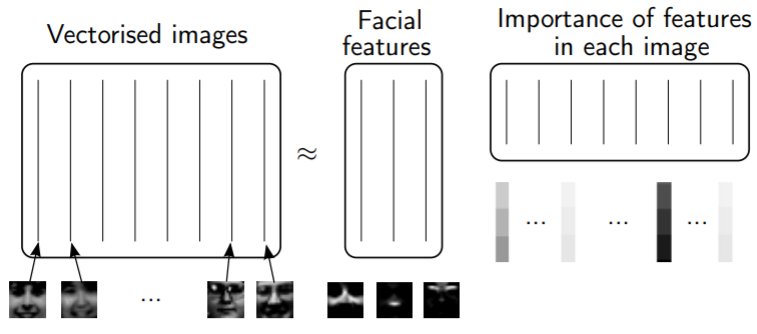
\includegraphics[width=0.6\textwidth]{figure_man/pixel.png}
\end{center}

\vfill
\begin{footnotesize}
$^{(*)}$ Example from \url{http://perso.telecom-paristech.fr/~essid/teach/NMF_tutorial_ICME-2014.pdf}
\end{footnotesize}

\framebreak

\textbf{(Possible) Advantages: }
\begin{itemize}
\item The dimension reduction reveals \textbf{latent variables} (here: "Facial Features") and the data can be "explained".
\item The storage space can be reduced significantly (for appropriate choice of $k$). Instead of a $m \times n$ matrix, a $m \times k$ and a $k \times n$ matrix with $k \ll m, n$ must be stored. \\
\begin{footnotesize}
\vspace*{0.2cm}
Calculation example: $n = 1000$ images with $m = 10000$ pixels each. Using a matrix approximation of rank $10$ the storage space can be reduced from $m \times n = 1 \times 10^6$ to $m \times k + k \times n = 10000 \cdot 10 + 10 \cdot 1000 = 110000$ (about $10\%$ of the original size).
\end{footnotesize}
\vspace*{0.2cm}
% \item Geeignete Algorithmen könnten auch direkt auf $\mathbf{H}$ operieren.
\end{itemize}


% % \begin{itemize}
% % \item Für $n=100$ Bilder der Auflösung $400 \times 600 = 240.000$ Pixel hätte die Matrix
% % $$
% % 24 \cdot 10^6 \text{  Einträge}
% % $$
% % \item Könnten wir $\mathbf{X}$ mit einer Niedrigrangapproximation für $k = 3$ „gut“ annähern, so müssen bei der Speicherung von $\mathbf{W}$ und $\mathbf{H}$ insgesamt nur
% % $$
% % m \cdot k + k \cdot n = 100 \cdot 3 + 3 \cdot 240.000 = 720.300
% % $$
% % Einträge abgespeichert werden.
% % \end{itemize}


\framebreak

\textbf{Introductory Example 2:} Text mining

\lz

Given is a $m \times n$ document-term matrix $\mathbf{X}$, where

$$
x_{ij} = \text{Frequency of term $i$ in document $j$}
$$

Using a low-rank approximation, we approximate $\mathbf{X}$ with

$$
\mathbf{X} \approx \mathbf{W} \mathbf{H}
$$

Suppose we want to display various newspaper articles in a document-term matrix.

\begin{center}
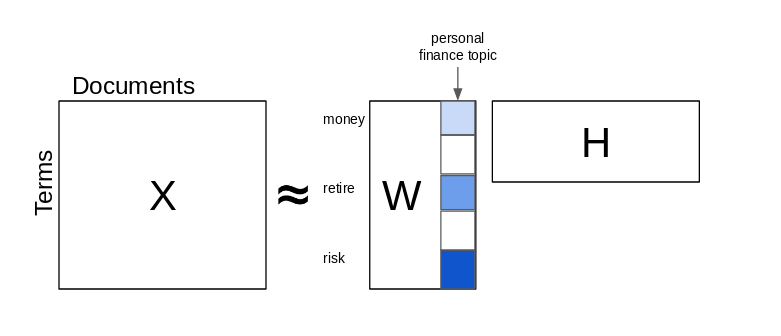
\includegraphics[width=0.7\textwidth]{figure_man/matrixapproxi_s8.png}
\end{center}

The $k$ columns in $\mathbf{W}$ represent different topics, and the entries of $\mathbf{W}$ can be interpreted as

$$
w_{ij} = \text{connection of word } i \text{ and subject } j
$$

\begin{center}
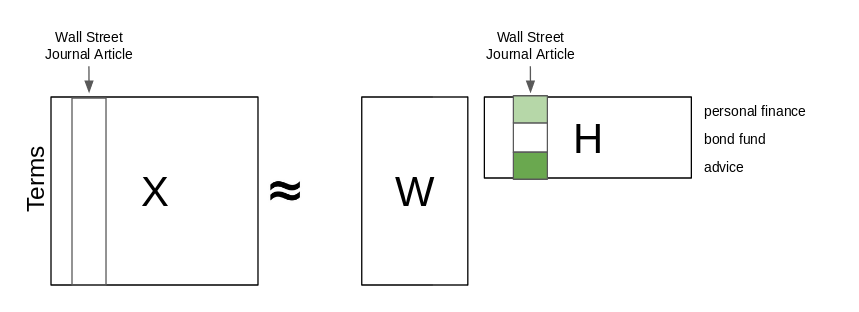
\includegraphics[width=0.7\textwidth]{figure_man/matrixapproxi_s9.png}
\end{center}

The entries of $\mathbf{H}$ can be interpreted as

$$
h_{ij} = \text{Measure for how much article } j \text{ discusses topic } i
$$

\framebreak

For fixed $k$ this can be formulated as a general optimization problem

$$
\min_{\mathbf{W} \in \R^{m \times k}, \mathbf{H} \in \R^{k \times n}} \|\mathbf{X} - \mathbf{WH}\|^2_F
$$

\lz

The Eckart-Young-Mirsky theorem states that the solution of the optimization problem is given by the \textbf{truncated singular value decomposition}

$$
\mathbf{X} \approx \bm{W} \bm{H} = \mathbf{U}_k \boldsymbol{\Sigma}_k\mathbf{V}_k^\top
$$

where matrix $\boldsymbol{\Sigma}_k$ contains the $k$ largest \textbf{singular values} and the matrices $\mathbf{U}_k$, $\mathbf{V}_k$ contain the corresponding \textbf{singular vectors} of $\mathbf{X}$. 

\lz 

The matrices $\bm{W}$ and $\bm{H}$ can be set as $\bm{W}:= \mathbf{U}_k \boldsymbol{\Sigma}_k$ and $\bm{H}:= \mathbf{V}_k^\top$ or as $\bm{W}:= \mathbf{U}_k (\boldsymbol{\Sigma}_k)^{1 / 2}$ and $\bm{H}:= (\boldsymbol{\Sigma}_k)^{1 / 2}\mathbf{V}_k^\top$. 

\end{vbframe}



\endlecture
\end{document}






